%\documentclass[a4paper,11pt]{article}
\documentclass[a4,12pt]{article}

\usepackage[utf8]{inputenc}
  \usepackage{amsmath,amsthm, amssymb, latexsym, graphicx,bbm,MnSymbol}
  \usepackage{xcolor}

\usepackage[colorlinks = true,
            linkcolor = blue,
            urlcolor  = blue,
            citecolor = blue,
            anchorcolor = blue]{hyperref}

\usepackage{natbib}
\bibliographystyle{elsarticle-harv}
\let\oldthebibliography=\thebibliography
\let\endoldthebibliography=\endthebibliography
\renewenvironment{thebibliography}[1]{%
    \begin{oldthebibliography}{#1}%
    \setlength{\parskip}{0ex}%
    \setlength{\itemsep}{0ex}%
}%
                 {%
  \end{oldthebibliography}%
                 }


%opening
\title{Accurate solutions of highly oscillatory systems under large time steps using higher-order phase averages}
\author{Werner Bauer, Colin J. Cotter}

\newcommand{\bla}{\Big\langle}
\newcommand{\bra}{\Big\rangle}
\newcommand{\dede}[2]{\frac{\delta #1}{\delta #2}}
\newcommand{\df}{\mathrm{d}} % differential operator
\newcommand{\sdbt}{\boldsymbol{\sigma} \df \boldsymbol{B}_t} % random velocity  
\newcommand{\curl}{\mathrm{curl}}
\newcommand{\dd}[2]{\frac{\diff#1}{\diff#2}}
%\newcommand{\dt}[1]{\diff\!#1}
\DeclareMathOperator{\diff}{d}

\newtheorem{theorem}{Theorem}
\newtheorem{definition}[theorem]{Definition}
\newtheorem{proposition}[theorem]{Proposition}
\newtheorem{corollary}[theorem]{Corollary}
\newtheorem{remark}[theorem]{Remark}
\newtheorem{lemma}[theorem]{Lemma}
\newcommand{\code}[1]{{\ttfamily #1}} 
\usepackage[margin=2cm]{geometry}


\newcommand{\checkit}[1]{{\color{red}#1}}
\newcommand{\werner}[1]{{\color{blue}#1}}
\newcommand{\incl}[1]{{\color{magenta}#1}}
  
%%% Todo
\newcommand{\todo}[1]{\vspace{5 mm}\par \noindent
\framebox{\begin{minipage}[c]{0.95 \textwidth}
\tt #1 \end{minipage}}\vspace{5 mm}\par}




\newcommand{\comments}[1]{{\color{gray!50}#1}}
\newcommand{\cyan}[1]{{\color{cyan}#1}}
\newcommand{\inred}[1]{{\color{red}#1}}
\newcommand{\ingreen}[1]{{\color{blue}#1}}
\newcommand{\red}{\color{red}}
\newcommand{\black}{\color{black}}
\newcommand{\yellow}{\color{yellow}}
\newcommand{\blue}{\color{blue}}



%%%


\newcommand{\xcirc}[1]{\vcenter{\hbox{$#1\circ$}}}
\renewcommand*{\Omega}{\varOmega} % fluid domain
\newcommand{\bord}{\partial\Omega} % boundaries
\newcommand{\sub}{\scriptscriptstyle} % smaller subscript
%\renewcommand*{\boldsymbol}{\boldsymbol} % vector in bold
%\newcommand{\df}{\mathrm{d}} % differential operator
\newcommand{\dt}{\df t} % timestep
\newcommand{\sdf}{\underline{\df}} % Stratonovich differential operator
\newcommand{\pdbt}{\varphi \df B_t} % random streamfunction
\newcommand{\spdbt}{\varphi \sdf B_t} % Stratonovich random streamfunction 
%\newcommand{\sdbt}{\boldsymbol{\sigma} \df \boldsymbol{B}_t} % random velocity  
\newcommand{\sdbth}{\boldsymbol{\sigma}_{\sub H} \df \boldsymbol{B}_t} % horizontal comp.
\newcommand{\sdbtz}{\sigma_{\sub z} \df B_t} % vertical comp.
\newcommand{\dpt}{\df p_t^{\sigma}} % random pressure
\newcommand{\Df}{\mathrm{\mathbb{D}}} % material differential operator
\newcommand{\Dfh}{\mathrm{\mathbb{D}}^{\sub H}}
\newcommand{\bdot}{\boldsymbol{\cdot}} % inner product
\newcommand{\grad}{\boldsymbol{\nabla}} % gradient operator
\newcommand{\gradh}{\boldsymbol{\nabla}_{\sub H}}
\newcommand{\tp}{^{\scriptscriptstyle T}} % matrix transport
\newcommand{\defin}{\stackrel{\scriptscriptstyle\triangle}{=}} % math definition
\newcommand{\gradp}{\boldsymbol{\nabla}^{\sub\perp}} % perp gradient operator
\newcommand{\jacobi}{\mathrm{J}} % Jacobi operator
\newcommand{\Exp}{\mathbb{E}} % Expectation
\newcommand{\Var}{\mathrm{Var}} % Variance
\newcommand{\tr}{\mathrm{tr}} % trace of matrix
\renewcommand*{\div}{\boldsymbol{\nabla\cdot}} % divergence operator
\newcommand{\divh}{\boldsymbol{\nabla}_{\sub H}\boldsymbol{\cdot}}
%\newcommand{\curl}{\boldsymbol{\nabla} \times} % curl operator
\newcommand{\adv}{\boldsymbol{\cdot\nabla}} % advection operator
\newcommand{\advh}{\bdot\boldsymbol{\nabla}_{\sub H}}
\newcommand{\laplac}{\nabla^{2}} % Laplacian operator
\newcommand{\bilaplac}{\nabla^{4}} % bi-Laplacian operator
\newcommand\Ro{\mbox{R}_{\mbox{o}}}  % Rossby number
\newcommand\Rb{\mbox{R}_{\beta}} % beta-Rossby number
\newcommand{\alf}{\frac{1}{2}} % one half
\newcommand{\real}{\mathbb{R}} % space of real number 
\newcommand{\Id}{\boldsymbol{\mathrm{I}}} % identity matrix
\newcommand{\KE}{\text{KE}}
\newcommand{\PE}{\text{PE}}
\newcommand{\E}{\text{E}}
\newcommand{\bfu}{{\bf u}}


\def\MM#1{\boldsymbol{#1}}
\newcommand{\pp}[2]{\frac{\partial #1}{\partial #2}} 
%\newcommand{\dede}[2]{\frac{\delta #1}{\delta #2}}
\def\MM#1{\boldsymbol{#1}}
% \DeclareMathOperator{\diff}{d}
% \DeclareMathOperator{\Tr}{Tr}
% \DeclareMathOperator{\uu}{\MM{u}^\delta}
% \DeclareMathOperator{\F}{\MM{F}^\delta}
% \DeclareMathOperator{\D}{D^\delta}
% \DeclareMathOperator{\q}{q^\delta}
% \DeclareMathOperator{\Z}{Z^\delta}
% \DeclareMathOperator{\qr}{\mathring{q}^\delta}
% \DeclareMathOperator{\DIV}{DIV}


\def\below#1#2{\mathrel{\mathop{#1}\limits_{#2}}}

\newcommand{\V}{\mathbf{V}}
\newcommand{\U}{\mathbf{U}}
\newcommand{\W}{\mathbf{W}}
\newcommand{\M}{\mathrm{M}}
\newcommand{\R}{\mathrm{R}}
\newcommand{\La}{\mathrm{L}}
\newcommand{\Fu}{\mathbf{F}}
\newcommand{\D}{\mathbf{D}}
\newcommand{\N}{\mathbf{N}}


\newcommand{\tN}{\tilde{N}}
\newcommand{\tk}{\tilde{k}}

\newcommand{\ob}[1]{$\mathcal{O}#1$}

\newcommand{\opL}{\mathcal{L}}
\newcommand{\opN}{\mathcal{N}}




\begin{document}

\maketitle


\begin{abstract}
We introduce a time integrator for a prototype model of highly oscillatory PDEs that exhibits accurate solutions even under the usage of large time step sizes. To achieve large time steps, we apply a phase averaging technique that smooths out the fast waves from the system. To avoid the errors that such smoothing usually entails, we use a higher order (HO) phase averaging algorithm based on the idea of Bauer et al. 2022. %\cite{Bauer22}.
This algorithm expresses the sensitivity of the solutions on the phases in terms of an HO basis which the equations are projected onto. The resulting HO phase corrections reduce the errors in the solutions even for finite averaging windows. Rather than using monomials as such HO basis as originally suggested in Bauer et al 2022, %\cite{Bauer22},
here we introduce an alternative basis in terms of exponentials and we discuss its properties.

Similarly to Bauer et al. 2022, %\cite{Bauer22},
we test this idea on an ODE describing the dynamics of a swinging spring, a model due to Peter Lynch. Although idealized, this model shows an interesting analogy to geophysical flows as it exhibits a high sensitivity of small scale oscillation on the large scale dynamics. On this example, we illustrate that the HO phase averaging method with an exponential basis allows for highly accurate solutions even when using large averaging windows and hence larger time step sizes than standard methods. These HO phase corrections (the reason for this improvement) can be evaluated independently, hence computed in parallel. In contrast, in standard averaging approaches, e.g. Peddle et al. 2019, % \cite{peddle2019parareal},
arbitrarily accurate solutions could only be obtained with small averaging windows as well as small time step sizes.  We present these highly promising results and discuss challenges in generalizing them to highly oscillatory PDEs for applications in simulations of weather, ocean, and climate.

\end{abstract}


\section{Introduction}

\begin{itemize}
 \item There is a need for new time integrators that benefit from the massively parallel supercomputer architectures and produce accurate solutions fast
 \item this is because new hardware gets more and more parallel, so to achieve speedup, PinT methods have to be developed
 \item PinT methods have various flavours, some of them use large time steps and parallelize the substeps required to be able to have such large time steps, hence they follow a parallel across the method ansatz. This has been done HERE...
 \item In some cases, this has lead to significant speedup, see e.g. Peddles, Hiroe, Colin
 \item The latter method share the fact that they use averaged equations in order to smooth over the fast equations (hence make them less stiff) which allows for an easier solving.
 \item However, as shown in Peddles, Hiroe, standard averaging methods introduce errors in the solutions that can only be avoided when both the averaging window as well as the time step size gets small.
 \item Unfortunately, this is in contrast to the original idea have a large time step via large averaging windows to gain efficiency.
 \item In this context, Bauer et al. 2022 introduces a novel pathway of how this diametral properties can be overcome. The idea is to allow for large averaging window that should entail large time steps, but add correction terms that increase accuracy.
 \item The derivation of the corrections is based on the understanding that we can parametrize the phase dependency of the solution in terms of a basis of this phase, which introduces phase averaging corrections.
 \item In Bauer 22 we have shown that this indeed leads to much more accurate solutions even under finite averaging windows
 \item HERE, extending the results of Bauer 22, here we introduce a new basis that allows for significantly larger averaging windows and much larger time steps while keeping the solution arbitrarily accurate
 \item Further, by developing an iterative SDC method, we introduce an iterative algorithm that avoids the inversion of the phase averaging matrix to be ready for going to SDEs
 \item The paper is structured as follows.
 In Section 2, we review the HO phase averaging idea which is based on coordinate transformed (by an exponential integral factor) form of the original PDE over which that fast waves can be smoothed out.

 In Section 3, we introduce a novel exponential basis to represent the equations phase dependency and determine the integral coefficients analytically, leading us to a HO phase averaged system for the swinging spring ODEs. The latter will also be briefly introduced here.

 In Section 4, we develop an iterative time stepping algorithm based on the SDE method that also introduces a block diagonalization of the original dense HO phase averaging matrix. This avoids the requirement to invert the latter matrix which might be dense in the case of PDEs to which we aim towards for future work (so we want to be prepared for this transition).

 In Section 5, we run numerical test with a focus on large averaging windows and time steps and if our algorithm can keep the solutions accurate and the drift small.

 In Section 6, we draw some conclusions and provide an outlook of how this methods, here developed for an ODEs, should be extended for PDEs.



\end{itemize}


\section{Foundations of the higher order phase averaging technique}


The starting point for a phase averaged PDE describing a highly oscillatory system is the following equation:
$$ \pp{}{t} \U(t) = \opL\U(t) + \opN(\U(t)),$$
where $\opL$ is a linear operator (with purely imaginary eigenvalues) and $\opN$ is a nonlinear operator. Using $\V(t,s) = e^{-(t+s) \opL} \U(t,x)$, where a phase variable $s$ had been added \citet{Bauer22}, introduces a coordinate transformed version:
\begin{equation}\label{equ_gen_V_s}
 \pp{}{t} \V(t,s) = e^{-(t+s) \opL} \opN \left(e^{ (t+s) \opL} \V(t,s) \right).
\end{equation}
This leads to a one-parameter family of solutions $\V(t,s)$ that depend on the phase parameter $s$. This additional parameter (relative to the original formulation in
\citet{haut2014asymptotic}) gives us new freedom in how to proceed, for example, it allows us to interpret averaging approaches discussed in the introduction. Being interested at the solution $s=0$ to obtain the original PDE, the assumption that $\V(t,s)$ is insensitive to changes in $s$ leads to a
 \emph{standard phase averaged PDE} for the phase averaged velocity  $\overline{\V}$, as in \citet{haut2014asymptotic}, that reads
 \begin{equation}\label{equ_gen_V_int}
   \pp{}{t}  \overline{\V}( t) =
   \frac{1}{2T} \int_{-T}^{T} \rho(\frac{s}{T}) e^{- (t+s) \opL} \opN\left(e^{ (t+s) \opL}
   \overline{\V}(  t) \right)  ds
\end{equation}
with finite averaging window $T$ an integral kernel $\rho$ with compact support, i.e.
\begin{equation}\label{normalization}
\frac{1}{2T}\int_{-T}^{T} \rho\left(\frac{s}{T}\right)ds=1.
\end{equation}
An important contribution of \citet{haut2014asymptotic} is to approximate the integral over $s$ by a sum. Each of the terms in this sum can be computed independently in parallel.

In \cite{Bauer22} we suggested a method that allowed us to obtain highly accurate solutions for large averaging windows $T$. The difference to current standard phase averaging methods is to parameterize the sensitivity of $s$ near $s = 0$ in a basis on which the equations are projected. This idea has been developed and tested on a prototype model of two resonating frequencies, which we will also use here in this work. This ansatz leads to \emph{higher order (HO) phase averaged systems} that feature \emph{HO phase corrections}. Only when the sensitivity of $s$ is represented through sufficiently many HO phase corrections, accuracy can be achieved. This result even explains why phase averaged equations in their current form entail significant errors. Namely, since we recover standard phase averaging \eqref{equ_gen_V_int} with zeroth order, we can conclude that the assumption of $\V(t,s)$ being insensitive to changes in $s$ causes these errors.



\paragraph{Step 1: Representation of HO phase averaged PDEs.}


We start with a suitable formulation of the HO phase averaged equations, namely from the averaged equation as in \eqref{equ_gen_V_int}. As suggested in my paper \cite{Bauer22}, we parameterize the dependency of the parameter $s$ around $s = 0$ by selecting a basis to represent this dependency and then project \eqref{equ_gen_V_int} onto it.
To this end, consider a $(2N+1)$-dim space spanned by the \emph{exponential basis} $\phi_k(s) = e^{k\opL s},  \inred{j = -N,...N}$, which allows us to expand the trial and test functions as
\begin{equation}\label{exp_basis}
\V(t,s) = \sum_{k = -N}^N \phi_k(s)\V_k(t) = e^{k\opL s} \V_k(t)
\end{equation}
and
\begin{equation}
\W(s)  = \sum_{j = -N}^N  \phi_j(s)\W_j  = e^{j\opL s} \W_j,
\end{equation}
respectively. Projecting \eqref{equ_gen_V_int} onto this space, we find the
\emph{HO phase averaged PDE}:
for all $\W_\inred{j}, \inred{j = -N,...N}$:
\vspace{-0.75em}
\begin{equation}\label{hoavgpde}
\begin{split}
\inred{\sum_{k=-N}^{N} }  \int_{-\infty}^{\infty}
&  \frac{e^{-\frac{s^2}{2T^2}}}{\sqrt{2\pi T^2}}
  \langle \W_\inred{j} , e^{(\inred{-j+k})\opL s}  \pp{}{t}  \V_\inred{k}(t) \rangle ds \\
 & = \inred{ \sum_{l,m =-N}^{N} } \int_{-\infty}^{\infty}
     \frac{e^{-\frac{s^2}{2T^2}}}{\sqrt{2\pi T^2}}
 \langle \W_\inred{j}, e^{(\inred{-j+l+m})\opL s}
 e^{-(t+s) \opL} \opN \left(e^{ (t+s) \opL}  {\V_\inred{l}}(t), e^{ (t+s) \opL} {\V_\inred{m}}(t)\right) \rangle ds
 \end{split}
\end{equation}\vspace{-0.75em}
\todo{let's use $\rho$ here, and not this gaussian, because it has no compact support,
so we specify the integral kernel later!!}
\noindent
where $\langle,\rangle$ denotes the inner product. We assume quadratic nonlinearity in $\V$
here (indices $l, m$), but higher nonlinearities are possible, too. The terms in red are related to the higher order parameterization of $s$. Note that for $k=0$, we recover \eqref{equ_gen_V_int} when setting $\overline{\V}(t):= \V_0(t)\forall t$. Note that rather than using the integral kernel \eqref{normalization} with compact support, we apply the following normalized Gaussian function:
\begin{equation}\label{normalization_gauss}
 \int_{-\infty}^\infty \frac{1}{\sqrt{2\pi T^2}} e^{-\frac{s^2}{2T^2}} ds = 1,
\end{equation}
as this will ease the analytical compuations of the integral values.

The general formulation \eqref{hoavgpde} permits us to explore other basis representations too. In \cite{Bauer22}, we used a monomial basis ($\phi_k(s) = s^k, k=0,...p$) for the swinging spring ODE of two resonating frequencies while in my ongoing research, I applied the exponential basis shown in \eqref{hoavgpde} for this ODE. Impressively, with increasing order, the averaged solution converges to a reference solution, however, for monomials the averaging window $T$ has to be still relatively small. Here, this study using an exponential basis exhibits similar accuracy but for much larger time steps. In both cases, we determine analytical expressions for the integrals and avoid hence errors due to integral approximations. This allowes us to better see the error reduction due to the HO phase corrections. However, in general, these integrals have to be approximated numerically, which is subject of future work.




\paragraph{Step 2: Numerical approximation of integrals.}

% To determine the analytical integral expressions for eqn???, we follow the approach of \citet{Bauer22}. ...
% \vspace{6em}
% \todo{What to do here???
% Mention computation of integrals also for exponential basis
% }
%\red
%\textbf{Remark (numerical computation of integrals)}
Because analytical expressions for the integrals in \eqref{hoavgpde} are hard to derive, we have to approximate them numerically. To this end, we replace the integral with a Riemann sum using appropriate weights \ingreen{$w_{\tk}$} (numerical quadrature) and set \ingreen{$s_{\tk} = \tk T/\tN$} where \ingreen{$\tN$} is the number of quadrature nodes. This leads to the approximation: for all $\W_\inred{j}, \inred{j = -N,...N}$:
\vspace{-0.75em}
\begin{align*}
\inred{\sum_{k=-N}^{N} }
\Bigg[
& \ingreen{\sum_{\tk=-\tN}^{\tN} w_{\tk}}
  \frac{e^{-\frac{\ingreen{s_{\tk}}^2}{2T^2}}}{\sqrt{2\pi T^2}}
  \W_\inred{j}  e^{(\inred{-j+k})\opL\ingreen{s_{\tk}}}
  \Bigg]
  \pp{}{t}  \V_\inred{k}(t) \\
 & = \inred{ \sum_{l,m =-N}^{N} }
 \Bigg[
 \ingreen{\sum_{\tk=-\tN}^{\tN} w_{\tk}}
     \frac{e^{-\frac{\ingreen{s_{\tk}}^2}{2T^2}}}{\sqrt{2\pi T^2}}
  \W_\inred{j} e^{(\inred{-j+l+m})\opL\ingreen{s_{\tk}}}
 e^{-(t+\ingreen{s_{\tk}}) \opL} \opN \left(e^{ (t+\ingreen{s_{\tk}}) \opL}  {\V_\inred{l}}(t), e^{ (t+\ingreen{s_{\tk}}) \opL} {\V_\inred{m}}(t)\right)   \Bigg].
 \end{align*}\vspace{-0.75em}

Through this numerical approximation of the integral, quadrature terms (blue) arise in the sums, additionally to the \emph{HO phase corrections} (red).

\black


Whether determined analytically or numerically, this system can be written in a  matrix-vector equation:
\vspace{-0.75em}
\begin{equation}\label{hoavg_mtx}
\inred{\sum_{k=-N}^{N} }
\M_\inred{j,k} \pp{}{t}  \V_\inred{k}(t) =
\inred{ \sum_{l,m =-N}^{N} } \mathbf{R}_\inred{j} ( \V_\inred{l} (t), \V_\inred{m}(t) ),
\ \inred{j = -N,...N},
\qquad \text{or} \ \ \M \pp{}{t}  \V = \mathbf{R} ,
\end{equation}\vspace{-1em}

\noindent
where the sum within the square brackets on the left-hand side gives the matrix element
$M_\inred{j,k}$ of $\M$ and on the right-hand side the element
$\mathbf{R}_\inred{j} ( \V_\inred{l}(t), \V_\inred{m}(t))$ of a nonautonomous forcing vector
$\mathbf{R}(t)$.

The system \eqref{hoavg_mtx} is a set of equations in which all solutions $\V_\inred{k}(t)$ are coupled via the matrix $\M$. $\V_\inred{0}(t)$ is the averaged solution we are interested in, but the coupling to the HO solutions $\V_\inred{k}(t),\forall k\neq0$ through \eqref{hoavg_mtx} results in the fact that $\V_\inred{0}(t)$ shows less error than standard averaging (i.e. $N=0$), at least for the ODE studied in \cite{Bauer22}.

\todo{Put also here an explicit representation (matrix vector form) for $N = 1$ for the system above.}





\paragraph{Step 3: Block diagonalization and SDC time discretization.} Using \eqref{hoavg_mtx} for PDEs, we face the challenge that they usually feature a full spectrum of frequencies, leading to a dense matrix $\M$ that couples all orders of velocities $\V_\inred{k}(t)$. For a small number of HO phase corrections, a direct solution of this system should still work, but for large numbers, this might get computationally very expensive. In the project, I will explore two possibilities: (i) to solve \eqref{hoavg_mtx} directly, or (ii) to use an iterative method that avoids inverting $\M$, introduced next. Note that $\M$ is unrelated to the usual mass matrix that arises from a FE discretization of the PDE of interest.


Because in the project we will use FE methods to discretize PDEs, FE mass matrices will enter the problem. In combination with implicit solvers, necessary for stiff PDEs as argued above, this leads to highly complex systems that are difficult to solve, especially for large problems such as weather and climate simulations.
The community is still searching for good strategies to solve those as monolithic systems, with only a few contributions, e.g. \cite{colinjemma2023}. But in general, direct approaches are prohibitively expensive and the usual approach is to use an iterative approach. This and the fact that we would like to have full control over the accuracy of the time solver is the reason why I plan to time-discretize \eqref{hoavg_mtx} with a flexible, higher order SDC method, for example.  \cite{Dutt2000, ruprecht2016,Speck18}. An advantage here is that the iterative SDC method can achieve an arbitrary order of accuracy by changing run-time parameters. We will exploit this flexibility when finding a balance between HO phase correction and SDC terms to obtain optimal performance and the highest accuracy.


SDC methods usually start from a Picard integral form of the PDE on hand. The occurring integral is approximated by a numerical quadrature, where different quadrature notes can be chosen, leading to a matrix formulation that is usually referred to as \emph{collocation problem}. However, this system of equations is dense and an attempt to solve it directly it is not advised \cite{Speck18}. However, with SDC this problem can be solved iteratively. In the literature, various realizations of SDC are discussed, for example, \cite{Speck18} introduces the SDC method as a preconditioned Picard iteration for the collocation problem, where the full collocation problem is solved as one system. The authors also suggested a parallelized version of this. This route can be followed too, probably at a later stage of the project and in collaboration with R. Speck and D. Ruprecht, but initially, I plan to develop an algorithm that solves the system iteratively over the collocation nodes point by point rather than in one go.



Considering these requirements, I next introduce a method that avoids inverting $\M$ by applying an iterative solving strategy instead. We start with splitting $\M$ into a diagonal $\mathbf{D}$ and an off-diagonal part $\mathbf{N}$ and formulate an
iterative method according to \cite{Abgrall16} to solve the following
block diagonalized (or lumped) system:
\vspace{-0.75em}
\begin{equation}\label{iter2sdc}
   \D \V^{j +1}_{k +1} =
          \M \V^{j + 1}_{k} \
        - \N \V^{j}_{k + 1}
                    + \Delta t_k \left[ \Fu(\V^{j+1}_{k}) - \Fu(\V^{j}_{k})\right]
                    + \Delta t \left[ \sum_{\alpha=1}^{N_t} \omega_{\alpha,k}\Fu(\V^{j}_\alpha) \right],
\vspace{-0.5em}
\end{equation}
where $j$ denotes the iteration index and $k$ the $N_t$ quadrature nodes of the SDC method with quadrature weights $\omega_{\alpha,k}$ \cite{Dutt2000} within the time interval $\Delta t = [t,t+1]$ and subintervals $\Delta t_k = [t_k,t_{k+1}]$.

\todo{Initialization of iteration of $j$, namely for $j=0$ we have $\V^{j+1}_{k=0} = \V^{j}_{k=0} = \V_n$
\checkit{CHECK!!!}}

This ansatz indeed bypasses the requirement to invert $\M$ while it simultaneously discretizes time with an SDC approach.
In case we have convergence, i.e. $|\V^{j + 1}_{k} - \V^{j}_{k}| \leq \epsilon$, the third term on the RHS vanishes and we are left with an implicit system that is solved with an SDC method ($\forall k, \V^{}_{k}$ without superscript indicates a converged value):
\vspace{-0.5em}
\begin{equation}\label{sdc_unlumped}
\M \V^{}_{k +1} =
   \M \V^{}_{k} + \Delta t \left[ \sum_{\alpha=1}^{N_t} \omega_{\alpha,k}\Fu(\V^{}_\alpha) \right]
\vspace{-0.5em}
\end{equation}
recalling $\M \V^{}_{k +1} = \D \V^{}_{k +1} + \N \V^{}_{k + 1} $. We refer to
\eqref{sdc_unlumped} as an \emph{unlumped system}. Note that for only one quadrature node (i.e. for ${N_t}=1$ we have $k=0,k+1 = t+1, \alpha =1$, hence $\omega_{1,0} = 1$, ending up with an implicit Euler backward scheme.
It is important to mention that the success of the work in \cite{Bauer22} was also based on the fact that HO solutions were reset at the end of each time step, i.e. $\V_k(t+1) =0, \forall k \neq 0$, which fully stabilized the solver. It is likely that this has to be done also in the case of PDEs.

So far, no specific model has been assumed, we only specified a quadratic nonlinearity for the sake of a clearer representation but higher order nonlinearities would also fit in the theory. To proceed, however, we have to select a model ODE or PDE and find a concrete representation of \eqref{iter2sdc}.


\section{Application of HO averaging technique to swinging spring}

The above framework is independent of a selection of ODE or PDE. It is intended to be applicable for PDEs, especially the block diagonalization addresses the case of dense HO mass matrices in case of PDEs. Here, we want to explore if HO terms using a novel exponential basis, instead of a monomial one as done in \cite{Bauer22}, has beneficial properties on an example of the swinging spring, as also used therein.

In this paper, we will compute the integrals of occuring in \eqref{hoavgpde} analytically, but the following methodology we are going to develop is equally valid if we used a numerical approximation as introduced in \eqref{hoavg_mtx}. Further, to ease the notation (and mimic those of \cite{Bauer22}), we introduce the following expression of the nonlinear RHS terms, a form that is shared by the swinging spring model we use here. That, we assume that the nonlinearity (here quadratic in $\V$ can be written as
\begin{equation}
 \sum_{\kappa} \Fu_{\kappa,l,m}(\V_l,\V_m) e^{i {(t + s) c_\kappa} }
  =   e^{-(t+s) \opL} \opN \left(e^{ (t+s) \opL}  {\V_{l}}(t), e^{ (t+s) \opL} {\V_{m}}(t)\right)
\end{equation}
which constitute of a sum over $\kappa$ of coefficients $ \Fu_{\kappa,l,m}(\V_l,\V_m)$ that depend quadratically on $\V$ and that are weighted with an exponential that depends on an additional parameter $c_\kappa$. The elaboration of this model in BAUER and the explicit representation of these coefficients in \cite{Bauer22} illustrates that this is a reasonable and useful way of writing the coordinate transformed (by $e^{-(t+s) \opL}$) nonlinear dynamics.

Using the basis for trial and test function as discussed above, we arive at the expension:
for $j = -N,..N$
 \begin{equation}\label{ho_avg_swingspring}
  \begin{split}
    \sum_{k = -N}^N
   &\int_{-\infty}^{\infty} \frac{e^{-\frac{s^2}{2T^2}}}{\sqrt{2\pi T^2}}
    e^{(-j+k)\opL s}  ds \ \pp{}{t}\V_k(t)   =  \\
  &      \sum_{\kappa} \sum_{l,m = -N}^N \Fu_{\kappa,l, m}(\V_l,\V_m) e^{i {t c_\kappa} }
  \int_{-\infty}^{\infty}\frac{e^{-\frac{s^2}{2T^2}}}{\sqrt{2\pi T^2}}
    e^{(-j + l + m)\opL s} e^{i {sc_\kappa} } ds
  \end{split}
 \end{equation}
This formulation allows us to find analytical expressions for the integral, as shown in the following proposition.
\begin{proposition}\label{prop_coeff}
The integrals on the LHS and RHS of equation~\eqref{ho_avg_swingspring} permit the following analytical expressions:
 \begin{align*}
 &  \frac{1}{\sqrt{2\pi T^2}}\int_{-\infty}^\infty e^{-\frac{s^2}{2T^2}}  e^{(-j+k)\opL s}  ds
  = e^{\frac{(-j + k)^2 \opL^2 T^2}{2}} =:\M_{jk} \\
 &   \frac{1}{\sqrt{2\pi T^2}}\int_{-\infty}^\infty e^{-\frac{s^2}{2T^2}}   e^{(-j+l+m)\opL s} e^{i {c_\kappa} s}  ds =  e^{\frac{(i {c_\kappa} + (-j+ l + m)\opL)^2 T^2}{2}} = :  \R_{j}^{\kappa lm}
 \end{align*}
with matrix elements $\M_{jk}$ of the $(2N+1) \times (2N +1)$-matrix $\M$ and $ \R_{j}^{\kappa lm}$ the $j$-th element of the $(2N+1)$-vector $ \R$.
\end{proposition}

\begin{proof}
We define $\beta$ that represents the operator $\beta = (-j +k)\opL$ for the first integral and $\beta = ((-j + l + m)\opL + i c_\kappa)$ for the second one. Using completion of the square for the powers of the exponents, namely
\begin{equation}
 -\frac{s^2}{2T^2} + \beta s =     - \frac{1}{2T^2} (s - \beta T^2)^2 + \frac{\beta^2 T^2}{2},
\end{equation}
both integrals can be cast in the following form
 \begin{equation}\label{prop_eqn1}
  e^{\frac{\beta^2T^2}{2}}\frac{1}{\sqrt{2\pi T^2}}\int_{-\infty}^\infty
  e^{- \frac{1}{2T^2} (s - \beta T^2)^2} ds.
 \end{equation}
Hence it is sufficent to integrate this general expression to find the desired result.

To proceed, we use the substitution $s' = s - \beta T^2$ with $ds' = ds$ and arrive at
 \begin{equation}\label{prop_eqn2}
  e^{\frac{\beta^2T^2}{2}}\frac{1}{\sqrt{2\pi T^2}}\int_{-\infty-\beta T^2}^{\infty-\beta T^2}
  e^{- \frac{1}{2T^2} (s')^2} ds'.
 \end{equation}
With $\opL$, hence $\beta$, being complex, the latter is a contour integral in the complex domain in which one term is integrated along the real axis and another one along a semi circle at infinity. Therefore, the shift of the real axis in the complex direction by $- \beta  T^2$
 does not change the integral value as long as there are no, or the same number of singularities
 enclosed by the contour (which is the case here).
 Therefore, we can equivalently write
\begin{equation}\label{prop_eqn3}
  e^{\frac{\beta^2T^2}{2}}\frac{1}{\sqrt{2\pi T^2}}\int_{-\infty}^{\infty}
  e^{- \frac{1}{2T^2} (s)^2} ds = e^{\frac{\beta^2T^2}{2}}
 \end{equation}
(skipping $'$ to ease notation) where we used the normalization \eqref{normalization_gauss}.
Upon resubstitution the corresponding values of $\beta$, this gives the integral value of the matrix element $jk$ in the first, and of the $j$-vector element in the second case while the dimensions of the matrix $\M$ and vector $ \R$ follow from \eqref{hoavg_mtx}. This finishes the proof.
\end{proof}


\begin{corollary}
The system \eqref{ho_avg_swingspring} can be cast in the matrix vector form \eqref{hoavg_mtx}, namely:
\begin{equation}\label{swingspring_mtx}
{\sum_{k=-N}^{N} }
\M_{jk} \pp{}{t}  \V_{k}(t) =
\sum_{l,m = -N}^N  \sum_{\kappa} \ \Fu_{\kappa,l, m}(\V_l(t),\V_m(t)) e^{i {t c_\kappa} }
\R_{j}^{\kappa lm}
\ {j = -N,...N},
\end{equation}
or, more compact as $\M \pp{}{t}  \V = \mathbf{R}$ with the coefficients defined as in Proposition~\ref{prop_coeff}.
\end{corollary}
\todo{Define $\mathbf{R}$ if the compact form is useful.}
\begin{proof}
 The formulation follows immediately from using the definitions of Proposition~\ref{prop_coeff}
 in \eqref{ho_avg_swingspring}.
\end{proof}



Next, we present an explicit representation of the system \eqref{swingspring_mtx}.
For $N = 1$ and $\opL = i \omega$ , the HO phase averaged equations for the swinging spring model read:
\begin{equation}\notag
 \begin{split}
 &
 \begin{pmatrix}
 1 & e^{\frac{- \omega ^2 T^2}{2}}  & e^{\frac{- 4\omega ^2 T^2}{2}}  \\
 e^{\frac{- \omega ^2 T^2}{2}} & 1   & e^{\frac{- \omega ^2 T^2}{2}} \\
 e^{\frac{- 4\omega ^2 T^2}{2}}    & e^{\frac{- \omega ^2 T^2}{2}} & 1   \\
 \end{pmatrix}
 \begin{pmatrix}
 \partial_t \V_{-1}(t)\\
 \partial_t \V_0(t)\\
 \partial_t \V_{+1}(t)\\
 \end{pmatrix}
  \hspace {0em} = \sum_{l,m = -N}^N  \sum_{\kappa} \ \Fu_{\kappa,l, m}(\V_l(t),\V_m(t)) e^{i {t c_\kappa} }
 \begin{pmatrix}
  e^{\frac{(i {c_\kappa} + (+1+l+m)\opL)^2 T^2}{2}}\\
  e^{\frac{(i {c_\kappa} + (0+l+m)\opL)^2 T^2}{2}}\\
  e^{\frac{(i {c_\kappa} + (-1+l+m)\opL)^2 T^2}{2}}\\
 \end{pmatrix}.
 \end{split}
\end{equation}




\blue

\section{Equations of the swinging spring}

As mentioned, ...




Let's start with the model equations. They read as follows:


\begin{scriptsize}
\hspace*{-1em}\begin{tabular}{ l| l | l | l}
   $c_m$ & $F^x_{m,k,l}$ &  $F^y_{m,k,l}$ & $F^z_{m,k,l}$   \\
   \hline \vspace{-1em}\\
  $c_1:= (\rho - 2)\omega_R$ & 0 & 0 & $F^z_{1,k,l} = c_z  (\hat X_{k} *\hat X_{l} + \hat Y_{k}*\hat Y_{l}) $ \\
  $c_2:= \rho \omega_R$ & $F^x_{2,k,l} = c_{xy}  \hat X_k *\overline{\hat Z}_l $ & $F^y_{2,k,l} = c_{xy}  \hat Y_k *\overline{\hat Z}_l $ & $F^z_{2,k,l} = 2 c_z (\hat X_k *\overline{\hat X}_l + \hat Y_k * \overline{\hat Y}_l)$ \\
  $c_3: =  (\rho + 2)\omega_R$ & $F^x_{3,k,l} = c_{xy}  \overline{\hat X}_k  *\overline{\hat Z}_l $ & $F^y_{3,k,l} = c_{xy}  \overline{\hat Y}_k  *\overline{\hat Z}_l $ &
      $F^z_{3,k,l} = c_z   (\overline{\hat X}_k *\overline{\hat X}_l + \overline{\hat Y}_k * \overline{\hat Y}_l)$ \\
  $c_4 := - \rho \omega_R$ &$F^x_{4,k,l} = c_{xy}  \hat X_k * \hat Z_l $ & $F^y_{4,k,l} = c_{xy}  \hat Y_k * \hat Z_l $ & 0 \\
  $c_5 := -(\rho + 2)\omega_R$ & $F^x_{5,k,l} = c_{xy}  \overline{\hat X}_k *\hat Z_l $  & $F^y_{5,k,l} = c_{xy}  \overline{\hat Y}_k *\hat Z_l $ & 0 \\
\end{tabular}
\end{scriptsize}

with coefficients $c_{xy} = 3  i  \omega_R\rho^2/16 $ and $c_z    = 3  i  \omega_R\rho/32$ (here $\rho = 2$).





\todo{here we need to put some equations that describe the swinging spring ODE}

\black



\newpage


 
 

\section{Numerical results}

The aim of this section is twofold. First, we investigate the use of the exponential basis to represent the phase dependency of the HO phase averaged form ??? and then we explore the SDC time method for the HO form with respect to preserving accuracy through higher order correction terms also for very large time steps.

\subsection{Investigation of the exponential basis}


Background on the use of odeint to set up and ideal environment for testing the impact of the higher order phase correction terms on the accuracy of the solutions relative to a filter reference solutions:
\begin{itemize}
 \item Idealized setup by using ODEint with adaptive time stepper to obtain accurate solution. Note: there is the sampling step, which is the interval in which the integrator returns results to you. This is controlled by you and usually you will select this equidistantly. And, there is the integration step, which is the discretization of time used by the integration algorithm. This is automatically adjusted to ensure that the (estimated) integration error agrees with the user defined error tolerances.

\item A comparison of phase averaged and original solutions requires us to filter (or smooth) the latter one, as it features the high frequency oscillations we want to get rid of in first place by using phase averaged equations. As it turns out, by choosing a large enough sampling step size serves as such filter, while the odeint solves then with the chosen accuracy relative to those sample points. \checkit{ADD Figure of this to explain what it means!!!}

In more details, when choosing for the given problem a sample size of $dt = 1$ with accuracy of about $1e-10$ for both atol and rtol, the integration step size is approximately $0.01$, but the solver returns a smoothed solutions where the fast oscillations are eliminated. In contrast, choosing a sampling of $dt = 0.01$ entails an integration time of again approximately $0.01$ but now, the higher oscillations are present.

\item This fact allows us to set up the following experiment. We compare the HO phase averaged soln. with the reference solution for a sampling step of $dt = 1$, hence a filtered reference solution. We also integrate the HO phase averaged ODE with same sampling step of $dt =1$ and same tolerance rtol and atol. Because ref is smoothed, the HO phase averaged with large averaging window $T>1dt$ will produce also solutions that do not have the high frequencies, hence we need the reference solution to be smoothed to obtain a high agreement between reference and HO solutions.

\item Further, because we integrate both HO phase averaged model and reference model with exactly the same time stepping method for the same accuracy and same sampling points and sampling steps, any difference between the solution should arise through the differences in the ODEs itself, not the time integration of those.

\item Also, errors that might result from using a large sampling step and the entailed smoothing (see figure), because we use the same time integration for both ODEs, this error would occur in both cases in the same way as we use the same sampling step size for both.


\todo{ADD FIGURE HERE about small and large sampling step of reference and some HO solutions.}



\end{itemize}

The experiment to test the accuracy of the HO form of the ODE:
\begin{itemize}
 \item We compute 2D error maps showing the relative time integrated L2 error between the reference solutions for sampling points $dt = 1$ and the HO soln also sampled at $dt =1$. For both ODE solvers, we have chosen rtol and atol to be 1e-10 in case 1 and 1e-13 in case 2
%  \checkit{ADD FIGURES}.
%  \checkit{Add l2 for x, y, z separately, but maybe combine them into one maximum error?}

\item The error is computed as follows.
\todo{ADD formula for time integrated L2 error}



 \item Figure~\ref{fig_error_maps_odeint} shows the time integrated relative L2 error between reference and HO solutions for values of various values of $N$ and $T$ for two solver tolerances. We see that for the suggested setup, the HO ode formulation converges almost up to the given time integrator solver tolerance, for the first row of solver tolerance $atol = rtol = 1e-10$ up to an error of about $1e-09$ and for the second row with $atol = rtol = 1e-13$ up to an error of about $1e-11$. In contrast to the results of \cite{Bauer22}, the use of the novel exponential basis does not show a dependency of this error of the choosen averaging window $T$, so here we can have larger $T$ (we also tested values larger than those shown, up to about 50).

\begin{figure}[h]\centering
\begin{tabular}{ccc}
 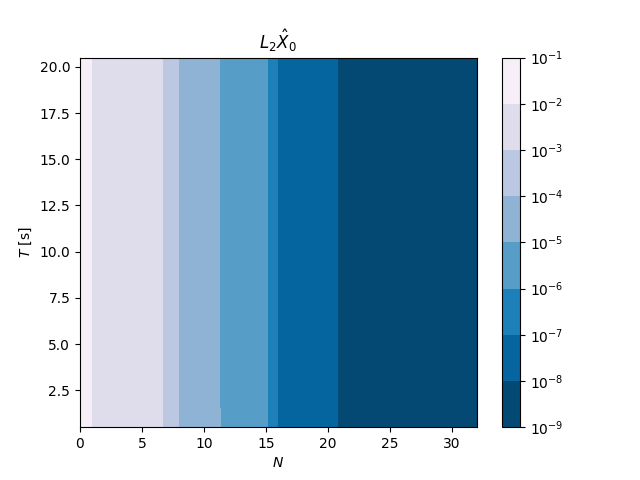
\includegraphics[scale=0.35]{figures/Figure_1.png} &
 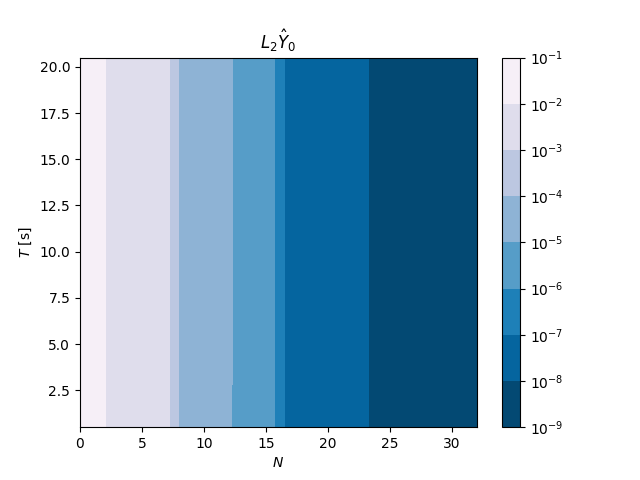
\includegraphics[scale=0.35]{figures/Figure_2.png} &
 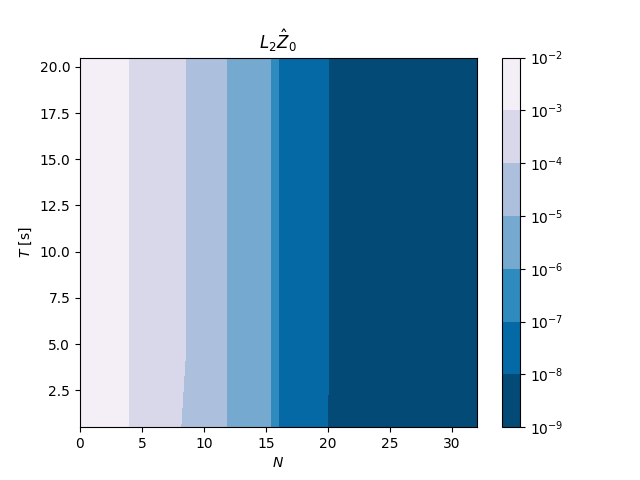
\includegraphics[scale=0.35]{figures/Figure_3.png} \\
 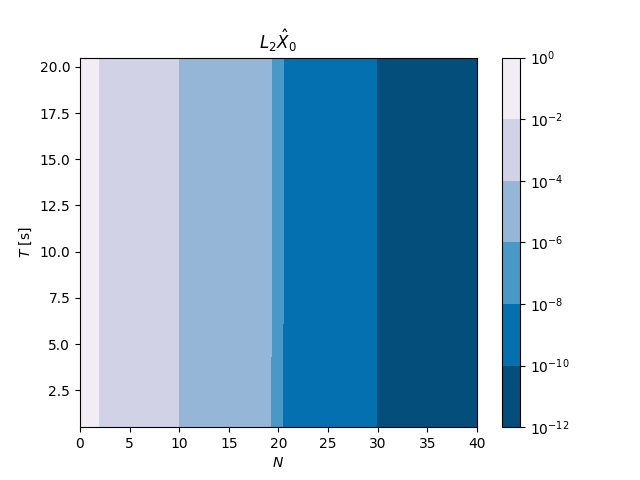
\includegraphics[scale=0.35]{figures/Figure_4.png} &
 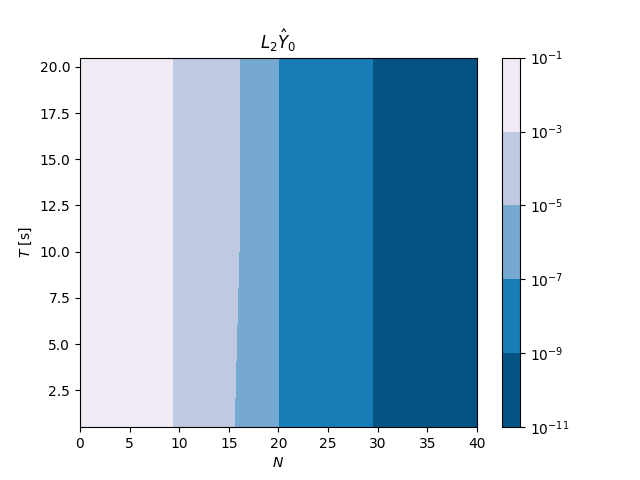
\includegraphics[scale=0.35]{figures/Figure_5.png} &
 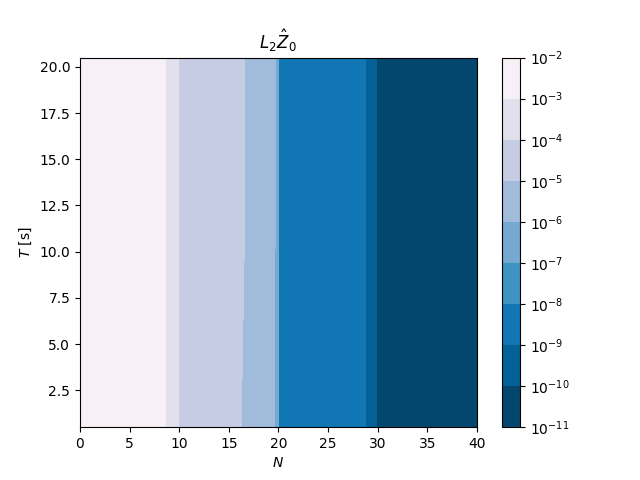
\includegraphics[scale=0.35]{figures/Figure_6.png}
\end{tabular}
\caption{Time integrated relative L2 error between reference and HO solutions for values of various values of $N$ and $T$. First row: solver tolerance for both ref and HO solvers of $atol = rtol = 1e-10$ and second row for
$atol = rtol = 1e-13$.
}
\label{fig_error_maps_odeint}
\end{figure}



\item This allows us conclude that the solutions of the HO phase averaged equations with exponential basis \eqref{exp_basis} converge for all values of $T >1 $ (up to the currently tested $T \approx 50$) to the solutions of the original modulated ODE.


\item The key here is that we use the same time integrator for both reference and HO model, hence reducing the error difference purely to the difference between the original and the HO phase averaged ODEs. As mentioned above, odeint, to achieve the desired accuracy, needs to have much smaller integration steps which, if we did not proceed from here, this would make our endeavour so far pointless because we wanted to have large time steps in first place.

\item In the next section, we test now the accuracy of our novel SDC solver for actually large time steps, that also feature substeps, but here they can be parallelized, providing us with the desired pathway for parallelization in time.


\end{itemize}







\subsection{Exporing the SDC method to obtain large time steps}







\newpage


\section{Colin's notes in tex}

\begin{equation}
jj 
\end{equation}



\todo{UPDATE bibiography}

% \bibliography{higher}
\begin{thebibliography}{17}
\expandafter\ifx\csname natexlab\endcsname\relax\def\natexlab#1{#1}\fi
\expandafter\ifx\csname url\endcsname\relax
  \def\url#1{\texttt{#1}}\fi
\expandafter\ifx\csname urlprefix\endcsname\relax\def\urlprefix{URL }\fi

\bibitem[{Abdulle et~al.(2012)Abdulle, Weinan, Engquist, and
  Vanden-Eijnden}]{abdulle2012heterogeneous}
Abdulle, A., Weinan, E., Engquist, B., Vanden-Eijnden, E., 2012. The
  heterogeneous multiscale method. Acta Numerica 21, 1--87.

\bibitem[{Ariel et~al.(2009)Ariel, Engquist, and Tsai}]{ariel2009}
  Ariel, G., Engquist, B., and Tsai, R. 2009. A multiscale method for highly oscillatory ordinary differential equations with resonance. Mathematics of Computation, 78~(266), 929-956.

\bibitem[{Ariel et~al.(2016)Ariel, Kim, and Tsai}]{ariel2016}
  Ariel, G., Kim, S. J., and Tsai, R. 2009. Parareal multiscale methods for highly oscillatory dynamical systems. SIAM Journal on Scientific Computing,
  38~(6), A3540--A3564.

\bibitem[{Babin et~al.(1997)Babin, Mahalov, Nicolaenko, and Zhou}]{Babin1997}
Babin, A., Mahalov, A., Nicolaenko, B., Zhou, Y., Jun 1997. On the asymptotic
  regimes and the strongly stratified limit of rotating boussinesq equations.
  Theoretical and Computational Fluid Dynamics 9~(3), 223--251.

\bibitem[{Bauer et~al.(2022)Bauer, Cotter, and Wingate}]{Bauer22}
???


\bibitem[{Caliari et~al.(2021)Caliari, Einkemmer, Moriggl, and
  Ostermann}]{CALIARI2021110289}
Caliari, M., Einkemmer, L., Moriggl, A., Ostermann, A., 2021. An accurate and
  time-parallel rational exponential integrator for hyperbolic and oscillatory
  pdes. Journal of Computational Physics 437, 110289.

\bibitem[{Charney et~al.(1950)Charney, Fjortoft, and von Neumann}]{ChFjNe1950}
Charney, J.~G., Fjortoft, R., von Neumann, J., 1950. Numerical {I}ntegration of
  the {B}arotropic {V}orticity {E}quation. Tellus 2, 237--254.

\bibitem[{Davies et~al.(2003)Davies, Staniforth, Wood, and
  Thuburn}]{Davies_etal_03}
Davies, T., Staniforth, A., Wood, N., and Thuburn, J., 2003. Validity of anelastic
  and other equation sets as inferred from normal-mode analysis. Quarterly
  Journal of the Royal Meteorological Society 129~(593), 2761--2775.

\bibitem[{Enquist and Tsai(2005)}]{enquist2005}Engquist, B., and Tsai, Y.. "Heterogeneous multiscale methods for stiff ordinary differential equations." Mathematics of computation 74.252 (2005): 1707-1742.
\bibitem[{Haut and Wingate(2014)}]{haut2014asymptotic}
Haut, T., Wingate, B., 2014. An asymptotic parallel-in-time method for highly
  oscillatory {PDE}s. SIAM Journal on Scientific Computing 36~(2), A693--A713.

\bibitem[{Haut et~al.(2016)Haut, Babb, Martinsson, and Wingate}]{haut2016high}
Haut, T.~S., Babb, T., Martinsson, P., Wingate, B., 2016. A high-order
  time-parallel scheme for solving wave propagation problems via the direct
  construction of an approximate time-evolution operator. IMA Journal of
  Numerical Analysis 36~(2), 688--716.

\bibitem[{Holm and Lynch(2002)}]{holm2002stepwise}
Holm, D.~D., Lynch, P., 2002. Stepwise precession of the resonant swinging
  spring. SIAM Journal on Applied Dynamical Systems 1~(1), 44--64.

\bibitem[{Jones et~al.(1999)Jones, Mahalov, and Nicolaenko}]{Jones1999}
Jones, D., Mahalov, a., Nicolaenko, B., 1999. {A Numerical Study of an Operator
  Splitting Method for Rotating Flows with Large Ageostrophic Initial Data}.
Theoretical and Computational Fluid Dynamics 13~(2), 143.

\bibitem[{Kevrekidis et~al.(2003)}]{Kevrekidis2003}
  Kevrekidis, I.~G., Gear, C.~W., Hyman, J.~M., Kevrekidis, P.~G. et al,
  2003. {Equation-free, coarse-grained multiscale computation: Enabling mocroscopic simulators to perform system-level analysis}. Communications in Mathematical Sciences, 1~(4), 715--762.

\bibitem[{Majda and Embid(1998)}]{majda1998averaging}
Majda, A.~J., Embid, P., 1998. Averaging over fast gravity waves for
  geophysical flows with unbalanced initial data. Theoretical and computational
  fluid dynamics 11~(3-4), 155--169.

\bibitem[{Minion(2011)}]{minion2011hybrid}
Minion, M., 2011. A hybrid parareal spectral deferred corrections method.
  Communications in Applied Mathematics and Computational Science 5~(2),
  265--301.

\bibitem[{Peddle et~al.(2019)Peddle, Haut, and Wingate}]{peddle2019parareal}
Peddle, A.~G., Haut, T., Wingate, B., 2019. Parareal convergence for
  oscillatory {PDE}s with finite time-scale separation. SIAM Journal on
  Scientific Computing 41~(6), A3476--A3497.

\bibitem[{Sanders et~al.(2007)Sanders, Verhulst, and Murdock}]{SandersVerhulst}
Sanders, J.~A., Verhulst, F., Murdock, J., 2007. Averaging methods in nonlinear
  dynamical systems, 2nd Edition. Applied mathematical sciences. Springer, New
  York, Berlin, Heidelberg.

\bibitem[{Schochet(1994)}]{schochet1994fast}
Schochet, S., 1994. Fast singular limits of hyperbolic pdes. Journal of
  differential equations 114~(2), 476--512.

\bibitem[{Schreiber et~al.(2018)Schreiber, Peixoto, Haut, and
  Wingate}]{schreiber2018beyond}
Schreiber, M., Peixoto, P.~S., Haut, T., Wingate, B., 2018. Beyond spatial
  scalability limitations with a massively parallel method for linear
  oscillatory problems. The International Journal of High Performance Computing
  Applications 32~(6), 913--933.

\bibitem[{Smith and Waleffe(2002)}]{SmithWaleffe2002}
Smith, L.~M., Waleffe, F., 2002. Generation of slow large scales in forced
  rotating stratified turbulence. Journal of Fluid Mechanics 451, 145--168.

\bibitem[{Tao et~al.(2010)Tao, Owhadi, and Marsden}]{tao2010}Tao, M., Owhadi, H., and Marsden, J. E., 2010. Nonintrusive and structure preserving multiscale integration of stiff ODEs, SDEs, and Hamiltonian systems with hidden slow dynamics via flow averaging. Multiscale Modeling and Simulation 8~(4), 1269-1324.

\bibitem[{Wingate et~al.(2011)Wingate, Embid, Holmes-Cerfon, and
  Taylor}]{wingate2011low}
Wingate, B.~A., Embid, P., Holmes-Cerfon, M., Taylor, M.~A., 2011. Low {R}ossby
  limiting dynamics for stably stratified flow with finite froude number.
  Journal of fluid mechanics 676, 546--571.

\end{thebibliography}









\end{document}













